% THIS IS SIGPROC-SP.TEX - VERSION 3.1
% WORKS WITH V3.2SP OF ACM_PROC_ARTICLE-SP.CLS
% APRIL 2009
%
% ----------------------------------------------------------------------------------------------------------------
% This .tex file (and associated .cls V3.2SP) *DOES NOT* produce:
%       1) The Permission Statement
%       2) The Conference (location) Info information
%       3) The Copyright Line with ACM data
%       4) Page numbering
% ---------------------------------------------------------------------------------------------------------------
% It is an example which *does* use the .bib file (from which the .bbl file
% is produced).
% REMEMBER HOWEVER: After having produced the .bbl file,
% and prior to final submission,
% you need to 'insert'  your .bbl file into your source .tex file so as to provide
% ONE 'self-contained' source file.
%

\documentclass[12pt, conference, compsocconf, letterpaper]{IEEEtran}
%\documentclass{sig-alternate}

%\usepackage{amssymb}
\usepackage{algorithmic,algorithm, graphicx}
\usepackage{paralist}
\usepackage{url}
\usepackage{authblk}
  
\newcommand{\dims}{\mathsf{d}}

%\DeclareMathOperator*{\argmin}{arg\,min}

\begin{document}

\title{INF5090/9090\\State Exchange in Distributed Applications}

%\subtitle{[Extended Abstract]
%\titlenote{A full version of this paper is available as
%\textit{Author's Guide to Preparing ACM SIG Proceedings Using
%\LaTeX$2_\epsilon$\ and BibTeX} at
%\texttt{www.acm.org/eaddress.htm}}}
%
% You need the command \numberofauthors to handle the 'placement
% and alignment' of the authors beneath the title.
%
% For aesthetic reasons, we recommend 'three authors at a time'
% i.e. three 'name/affiliation blocks' be placed beneath the title.
%
% NOTE: You are NOT restricted in how many 'rows' of
% "name/affiliations" may appear. We just ask that you restrict
% the number of 'columns' to three.
%
% Because of the available 'opening page real-estate'
% we ask you to refrain from putting more than six authors
% (two rows with three columns) beneath the article title.
% More than six makes the first-page appear very cluttered indeed.
%
% Use the \alignauthor commands to handle the names
% and affiliations for an 'aesthetic maximum' of six authors.
% Add names, affiliations, addresses for
% the seventh etc. author(s) as the argument for the
% \additionalauthors command.
% These 'additional authors' will be output/set for you
% without further effort on your part as the last section in
% the body of your article BEFORE References or any Appendices.

%\numberofauthors{3} %  in this sample file, there are a *total*
% of EIGHT authors. SIX appear on the 'first-page' (for formatting
% reasons) and the remaining two appear in the \additionalauthors section.
%
\author{
	Magnus Evensberget\\
	Institute of Informatics\\
	University of Oslo\\
	magnusev@ifi.uio.no
\and
	Vinay Setty\\
	Institute of Informatics\\
	University of Oslo\\
	vinay@ifi.uio.no
}

\maketitle
\begin{abstract}
This assignment is part of the Real-time Application Mobility Platform (TRAMP) project with focus on distributed multimedia applications with real-time requirements.
The goal of the assignment is to design and implement at least two components (producer and consumer) of a real-time application (such as a media player) and evaluate the provided distribution framework with respect to delay, throughput and other relevant metrics. Above is an overview of the provided framework. Your objective is to design and implement the producer and consumer application parts (the two gray components). The producer/consumer duo can run locally on one machine or be distributed over a network. In addition, multiple consumers can subscribe to the same produced data and receive identical copies.
\end{abstract}

% A category with the (minimum) three required fields
%\category{H.4}{Information Systems Applications}{Miscellaneous}
%A category including the fourth, optional field follows...
%\category{D.2.8}{Software Engineering}{Metrics}[complexity measures, performance measures]

%\terms{Design, Experimentation, Performance, Measurement}



\section{Introduction}
In our assignment we were to use the Real-time Application Mobility Platform (TRAMP). This is a project developed by the Distributed Multimedia Systems (DMMS) group at the University of Oslo.

This is a assignment given to us in the course INF5090 - Advanced Topics in Distributed Systems which is a course given by the University of Oslo, as well as Lancaster University in England and University of Mannheim in Germany. The teachers are Thomas Plagemann and Vera Goebel with their teaching assistants Piotr Kaminski and Hans Vatne Hansen. These are also the people that developed the TRAMP framework together with some other developers all from the University of Oslo.


\section{Related work}
\label{sec:relatedwork}

\subsection{Skype}

As we've mentioned earlier in the report Skype is one of the applications the developers of the TRAMP framework reference to. Skype was the first peer-to-peer voice over IP (VoIP) network, and requires minimal infrastructure in order to function. Skype came on market in late 2003 developed by Niklas Zennstr�m and Janus Friis, the two main developer behind the filesharing system Kazaa. this was bought by eBay in late 2005 and again by Microsoft in May 2011. Since Skype is propriatory, the code is not available and this is therefore based on observations and partial reverse engineering of the protocol.

\begin{figure}[hb]
%\centering
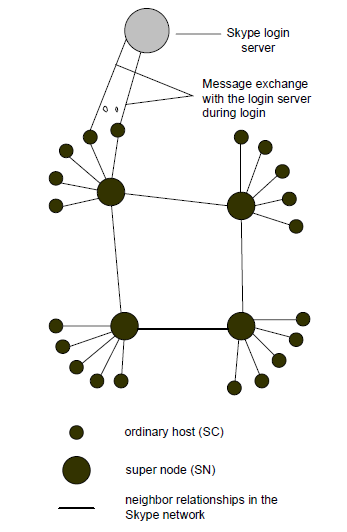
\includegraphics[width=200pt]{Skype_Architecture.png}
\caption{Picture of the skype arcitecture \cite{Analysis_of_Skype_p2p}}
\end{figure}

The skype arcitecture is designed around three entities: Supernodes, regular nodes and the login server (See fig. 1). Each regular node has a cache of the IP address and portnumber to all reachable Supernodes. The Supernodes are a subset of the regular nodes. If a node has high uptime, good bandwidth and is not restricted by firewalls or Network Address translation (NAT) it can be chosen as a Supernode\cite{Analysis_of_Skype_p2p}. This will ofcourse put some extra stress on the nodes not behind NAT, but also make Skype possible to work for free due to the little infrastructure needed in order to make the network work. Another issue for these Supernodes is that they are used as third party for UDP hole punching to connect clients behind NAT. UDP hole punching is done by letting the regular nodes behind NAT connect to the third party (the Supernode) thereby opening ports that they can use for direct traffic between the two regular nodes. This is only open as long as there is communication traffic going. If there is a prolonged absence of traffic Skype sends ``keep alive'' packets instead of closing the connection and then having to use the Supernode as a third party again redo the connection.\cite{UDP_holepunching}

This is something that might be implemented in TRAMP to scale up the network. 



%talk about a streaming application (pref p2p udp and tcp and what is trades / tradeoffs when using the different


\section{System Design}
\label{sec:design}

\begin{center}
\begin{figure*}[ht!]
 \centering
 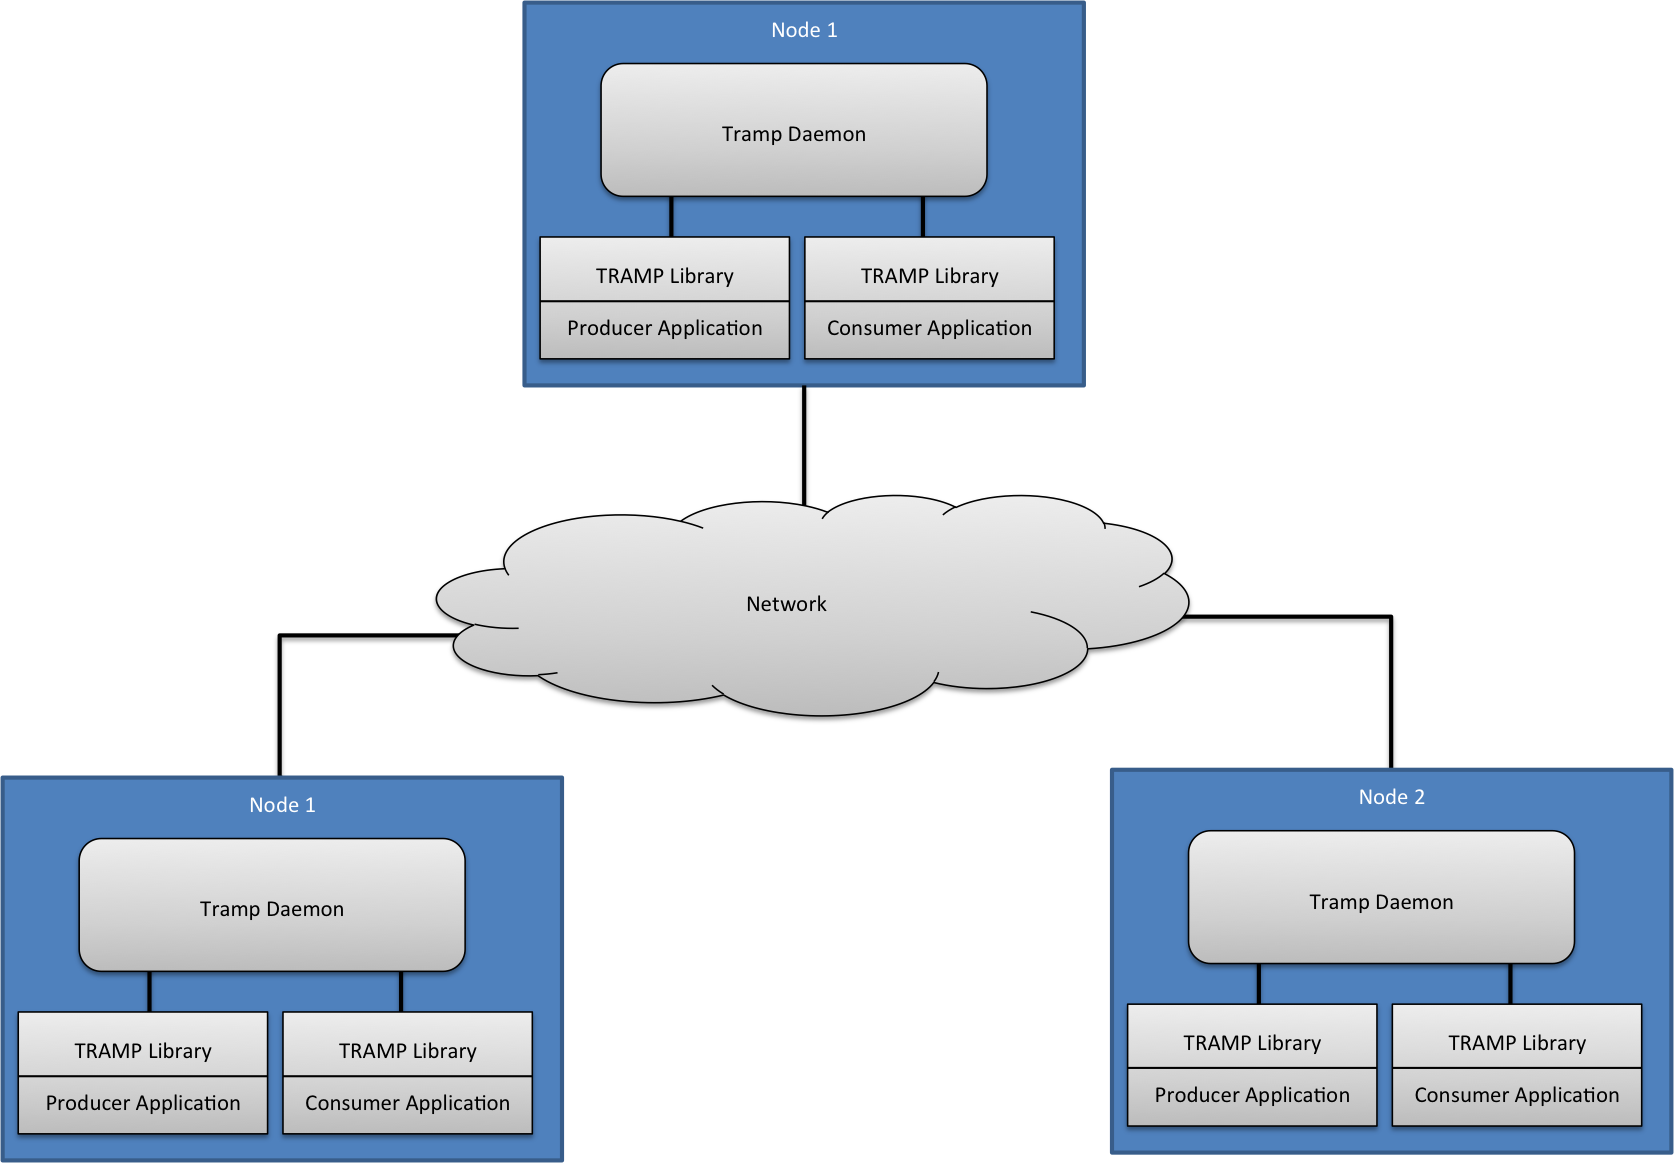
\includegraphics[width=6.0in, height=3.5in]{tramp_arch.png}
 %img1.pdf: 0x0 pixel, 300dpi, 0.00x0.00 cm, bb=
\caption{The TRAMP Architecture}
\end{figure*}
\end{center}

The TRAMP platform is a platform designed to stream real-time data from a device to other devices connected to the session, mobility is the keyword. Lets take the example given in the introduction; You are on a skype call with some of your friends when you find out you need to go out of the house. Traditionally you then had to end the skypecall and call them up using your phone. The goal for TRAMP is to be able to seamlessly enter the conversation without your friend noticing you just changed device.

In TRAMP this is done by having a TRAMP daemon running on each device, with a consumer and a producer. The producer produces data, putting it into the shared memory, the TRAMP daemon then pushes the data to all other daemons connected to this session. When a TRAMP daemon gets data it puts it into the shared memory so the consumer can read it. All nodes has a TRAMP daemon, a producer and a consumer running. The shared memory of all nodes in the session are in synch.




\section{The choice of streamer}
\label{sec:streamer}
When we got this assignement we had to look at what we would implement in order to test the TRAMP platform. In the sample code there was implemented a simple chat program, so we decided to implement something that streamed a lot of data. There are several ways to do this; we could make a file sharing system, an audio streaming application (like Skype) or a video streaming application. We decided on looking into FFMPEG.

FFMPEG is a complete cross-platform solution to record, convert and stream video and audio. It is a free software licensed under the LGPL or GPL (dependent on the configuration), and is the leading multimedia framework today.\cite{FFMPEG-homepage}
FFMPEG provides tools for converting, streaming, playing and analysing multimedia, as well as a full developers library with the possibility to create allmoast anything you want. Big projects such as QStream, VLC, GStreamer and Google Chrome has used the framework.

Due to time constraints we decided we did not have enough time to implement this framework. Instead we implemented a streamer that copied over one big file by chunking the big file into small bits, sending them and putting them back together on the other side. This will in our eyes show the capabilities of TRAMP just as well as a more sophisticated streamer like the FFMPEG solution we had planned.

\subsection{Our implementation}
To explain what we have done to the code, we must first talk about how the sample chat program work. We decided to use this as a base, as it had a lot of the code we needed. 
TODO:Get a better understanding of what we've done:TODO

\begin{figure*}[ht!]
\centering
 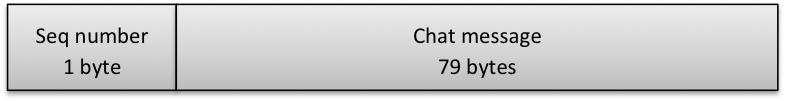
\includegraphics[width=300pt]{sendchatpkt.png}
 % sendchatpkt.png: 786x101 pixel, 150dpi, 13.31x1.71 cm, bb=0 0 377 48
\caption{Packet header for the chat application}
\label{Figure:Packet_header_chat}
\end{figure*}


\begin{figure*}[ht!]
\centering
 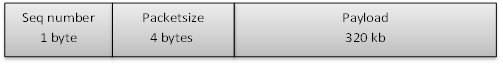
\includegraphics[width=300pt]{sendpkt.png}
 % sendchatpkt.png: 786x101 pixel, 150dpi, 13.31x1.71 cm, bb=0 0 377 48
\caption{Packet header for the file sending addon}
\end{figure*}

\begin{figure*}[ht!]
\centering
 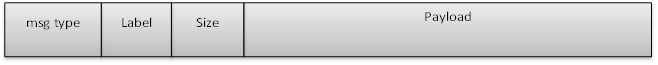
\includegraphics[width=300pt]{tramp_pkt.png}
 % sendchatpkt.png: 786x101 pixel, 150dpi, 13.31x1.71 cm, bb=0 0 377 48
\caption{TRAMP Daemon header}
\end{figure*}






\section{Proposed Optimizations}
\label{sec:optimizations}

\subsection{Shared Memory problem}
At the moment TRAMP is using shared memory in order to transfer data. TRAMP allocates 32mb

\subsection{Data transfer rate}
Pushing more data than the recieving nodes can pull

\subsection{Network topology}
atm mesh network, should be something else

\subsection{UDP vs TCP or both}




%shared mem probelm
%sending data to fast (recieving too slow)

%delay(?)

%udp vs tcp or both

\section{Evaluation}
\label{sec:eval}

\subsection{Experimental Setup}
Our implementation is a file sharer that uses the TRAMP platform to distribute files as described in Section \ref{sec:streamer}. We ran our experiments with one producer and 2 to 8 consumers. We ran all experiments on machines with Intel(R) Xeon(TM) CPU 3.20GHz quad core processors, 8GB RAM and connected with gigabit ethernet. For workload we send a 55MB movie file from the producers to the consumers. The packet size is limited to 320KB to mimic the real time video streaming bit rate. However, it is possible to read multiple chunks of 320KB and fill the 32MB limit of shared memory, which is not similar to a real time application. We sent the packets from producer with 100 milliseconds delay since without this delay the consumers could not process the data and lost some packets as the tramp daemon overwirtes the shared memory when the new packets arrive.

\subsection{Average Delay}
\begin{center}
\begin{figure*}[ht!]
 \centering
 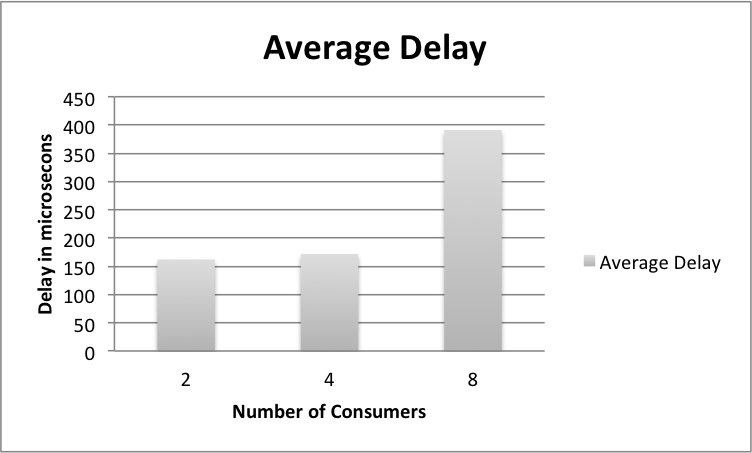
\includegraphics[width=4.0in]{avgdelay.png}
 %img1.pdf: 0x0 pixel, 300dpi, 0.00x0.00 cm, bb=
\caption{Average Delay Measurement}
\label{fig:delay}
\end{figure*}
\end{center}
We measure the average delay by sending the packet from producer and recording a timestamp $t_1$ before sending. For the sake of measuring the delay we reply the packet back to the sender with an ACK header. After the ACK packet is received the timestamp $t_2$ is noted again and the dealy is computed as the 
\[
 (t_2-t_1)/2
\]

. Since we ran experiments on machines connected with gigabit ethernet the network delay is negligible. The total delay is measured as the sum of processing delay at producer side, the network delay and the processing delay at consumer side. We denote the delays as below:
\begin{enumerate}
 \item Processing delay at producer: $PD$
\item Processing delay at consumer: $CD$
\item Network delay: $ND$
\end{enumerate}

The total delay is given by
\[
 PD + ND + CD
\]

In Figure \label{fig:delay} we show the average delay of sending packets from the producer to the consumer. The three parts of the delay $PD$, $CD$ and $ND$, are show in three stacks. We list the observations we made in the following:
\begin{enumerate}
 \item The $PD$ and $CD$ are almost constant for any number of consumers since it is local to each node
 \item The average network delay is the most varying 
 \item The difference between 2 consumers and 4 consumers is negligible (841 and 850 micro seconds). 
  \item In case of 2 consumers the producer sends the packets to consumers in 1 hop.
 \item In case of 4 consumers 2 of the consumers received packets in 1 hop and 2 consumers received packets in 2 hops, hence the difference is negligible.
\item However in case of 8 consumers the average delay significantly increases since there was consumer which received packets in 4 hops.
\end{enumerate}

The observations we made are due to the fact that the neighbors for dissemination of packets are chosen with minimum delay neighbors as described in Section \ref{nettop}.

\subsection{Packet Loss}
As described in Section \ref{smp} if the packet send rate is significantly fast (55MB in 40252 microseconds) results in around 88\% packet loss. Even though the network is reliable the loss is due to the fact the producer is significantly fast and consumer is significantly slow to process the packets. We did some measurements for packet loss with 100milliseconds delay before sending next packet, however the results we obtained were not meaningful due to some unkwnown problem. We omit the results in this paper due to lack of time. In Figure \ref{fig:delay} we show that with no delay between packets there is a packet loss of around 88\% and with 500ms delay between packets we were able to eliminate the packet loss to 0\%.
\subsection{Average Delay}
\begin{center}
\begin{figure*}[ht!]
 \centering
 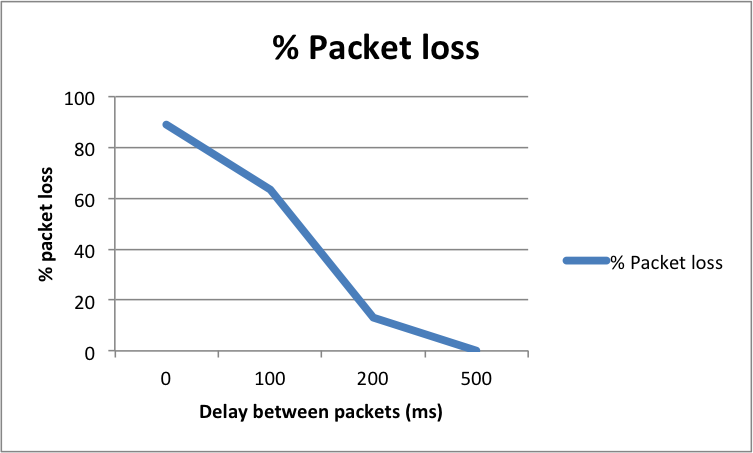
\includegraphics[width=4.0in]{packetloss.png}
 %img1.pdf: 0x0 pixel, 300dpi, 0.00x0.00 cm, bb=
\caption{Packet Loss Measurement}
\label{fig:pktloss}
\end{figure*}
\end{center}


\section{Conclusions}

%\section{Acknowledgments}



\bibliographystyle{abbrv}
\bibliography{main}  


%\balancecolumns

\end{document}
